\documentclass{article}
\usepackage[T1]{fontenc}
\usepackage[a4paper, total={6in, 11in}]{geometry}
\usepackage{algorithm}
\usepackage{algpseudocode}
\usepackage{float}
\usepackage{graphicx}
\usepackage{subcaption}

\def\v{0.47}

\title{%
	Obliczenia naukowe \\
	\large Lista 2}
\author{Szymon Janiak}
\begin{document}
\maketitle

\section*{Zadanie 1}
\subsection*{Opis problemu}
    Obliczenie iloczynu skalarnego róznymi funkcjami dwóch wektorów i porównanie wyników przy lekkiej zmianie danych wejściowych
\subsection*{Rozwiązanie}
    \begin{enumerate}
        \item "w przód" t.j. $\sum^n_{i=1} x_i y_i$
        \item "w tył" t.j. $\sum^1_{i=n} x_i y_i$
        \item "liczby dodatnie od najwiekszego do najmniejszego a ujemne na odwrót"
        \item "liczby ujemne od najwiekszego do najmniejszego a dodatnie na odwrót"
    \end{enumerate}
\subsection*{Wyniki}
    \begin{center}
        \begin{tabular}{|c|c|c|c|}
        \hline
            & Float64 stare dane & Float64 nowe dane & Prawidłowy wynik \\
            \hline\hline
            "1" & 1.0251881368296672e-10 & -0.004296342739891585 & -1.00657107000000e-11 \\
             \hline
             "2" & -1.5643308870494366e-10 & -0.004296342998713953 & -1.00657107000000e-11 \\
             \hline
             "3" & 0.0 & -0.004296342842280865 & -0.004296342842280865 \\
             \hline
             "4" & 0.0 & -0.004296342842280865 & -0.004296342842280865 \\
        \hline
        \end{tabular}
    \end{center}
\subsection*{Wnioski}
	Przy usunięciu ostatniej 9 z $x_4$ oraz ostatniej 7 z $x_5$ dostajemy różne wyniki dla podwójnej precyzji.
	Po tak lekkiej zmianie danych możemy zauważyć, że wyniki dla wszystkich funkcji są znacznie bardziej przybliżone, prawie identyczne.
	Dla Float32 nie ma żadnej różnicy, gdyż jest to za mała precyzja. Według definicji jest to źle uwarunkowane zadanie.

\section*{Zadanie 2}
\subsection*{Opis problemu}
	Narysować wykres funkcji $f(x) = e^xln(1 + e^{-x})$ w co najmniej dwóch dowolnych programach do wizualizacji. \\
	Porównać wykres funkcji z policzoną granicą dla funkcji $\lim_{x\to\infty}f(x)$.
\subsection*{Wyniki}
	\begin{figure}[H]
		\centering
		\begin{subfigure}[b]{\v\linewidth}
			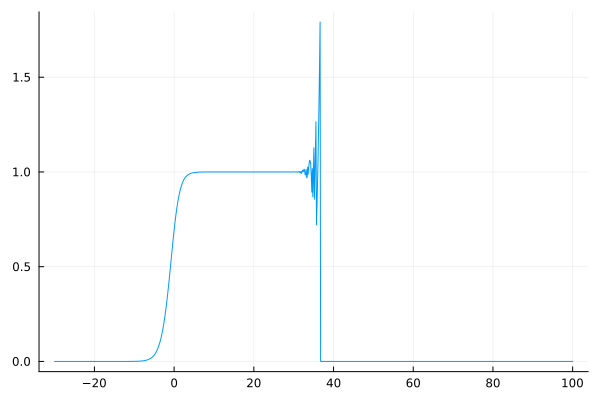
\includegraphics[width=\linewidth]{graphs/2.1.png}
			\caption{Biblioteka Plots w języku Julia}
			\label{fig:enter-label}
		\end{subfigure}
		\begin{subfigure}[b]{\v\linewidth}
			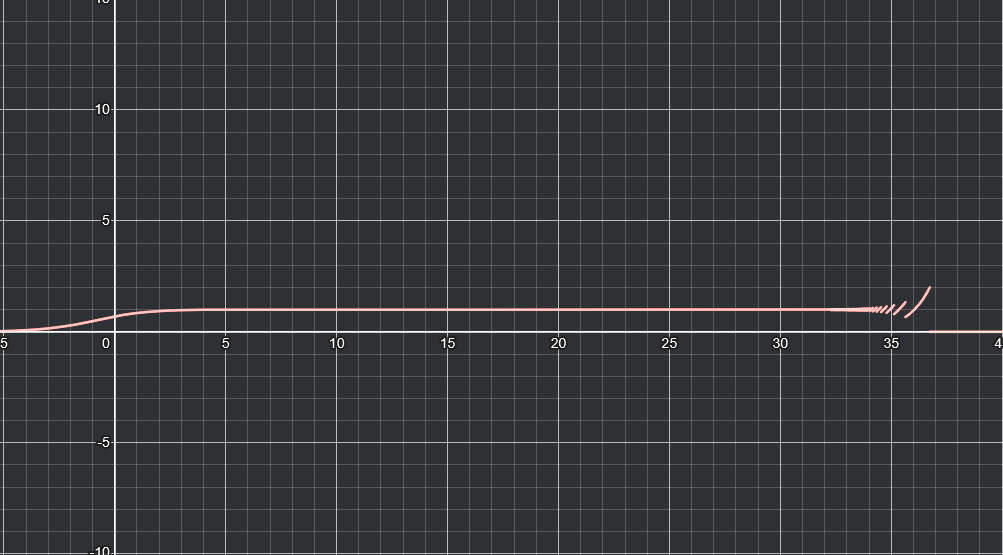
\includegraphics[width=\linewidth]{graphs/2.2.png}
			\caption{Desmos}
			\label{fig:enter-label}
		\end{subfigure}
	\end{figure}
	Poniżej policzona granica: \\
	\[\lim_{x\to\infty}e^xln(1+e^{-x})=\lim_{x\to\infty}\frac{ln(1+e^{-x})}{e^{-x}}=\lim_{x\to\infty}\frac{-e^{-x}}{(1+e^{-x})*(-e^{-e})}=\lim_{x\to\infty}\frac{1}{1+e^{-x}}=1\]

\subsection*{Wnioski}
	Widzimy na wykresach, że w okolicach $x = 30$ pojawiają się problemy z obliczaniem wartości naszej funkcji. \\
	Mimo, że funkcja dąży do 1 nasze programy mają wyraźny problem z obliczaniem wartości składających się na wynik naszej funkcji.
	Jest to prawdopodobnie spowodowane brakiem wystarczającej precyzji kiedy wartości $e^{-x}$ robią się coraz mniejsze.


\section*{Zadanie 6}
\subsection*{Opis problemu}
	Dla równania rekurencyjnego \\
	\centerline{$x_{n+1} := x_n^2 + c$ dla $n = 0, 1...,$ \\}
	Przeprowadzić następujące eksperymenty. Dla danych:
	\begin{enumerate}
        \item $c = -2$ i $x_0 = 1$
        \item $c = -2$ i $x_0 = 2$
        \item $c = -2$ i $x_0 = 1.99999999999999$
        \item $c = -1$ i $x_0 = 1$
        \item $c = -1$ i $x_0 = -1$
        \item $c = -1$ i $x_0 = 0.75$
        \item $c = -1$ i $x_0 = 0.25$
    \end{enumerate}
    wykonać w arytmetyce Float64, 40 iteracji podanego wyrażenia i przeprowadzić iteracje graficzną.
\subsection*{Wyniki}
	\begin{figure}[H]
		\centering
		\begin{subfigure}[b]{\v\linewidth}
			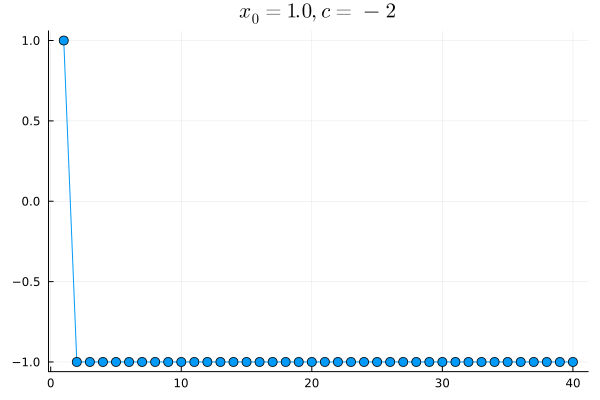
\includegraphics[width=\linewidth]{graphs/1.png}
		\end{subfigure}
		\begin{subfigure}[b]{\v\linewidth}
			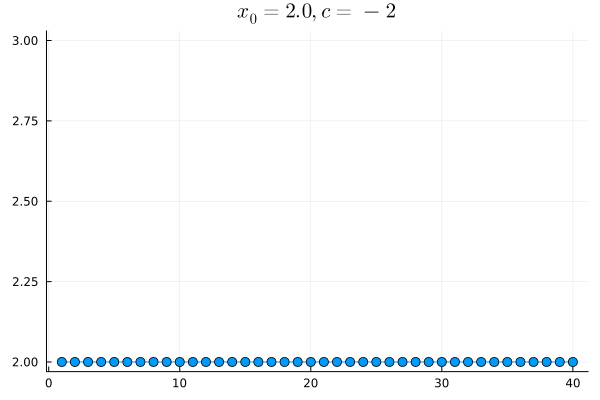
\includegraphics[width=\linewidth]{graphs/2.png}
		\end{subfigure}
		\begin{subfigure}[b]{\v\linewidth}
			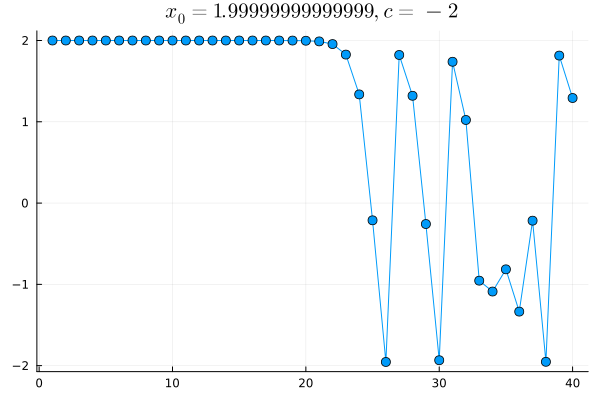
\includegraphics[width=\linewidth]{graphs/3.png}
		\end{subfigure}
		\begin{subfigure}[b]{\v\linewidth}
			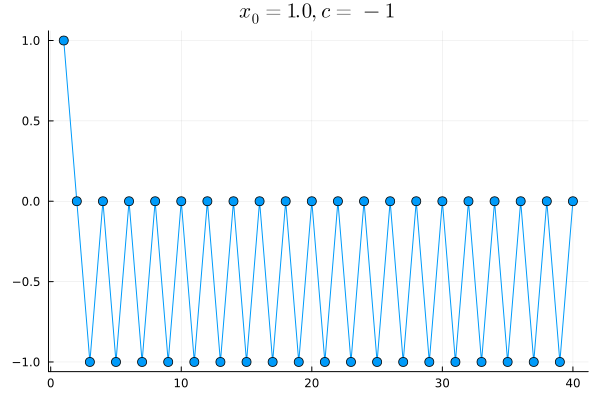
\includegraphics[width=\linewidth]{graphs/4.png}
		\end{subfigure}
		\begin{subfigure}[b]{\v\linewidth}
			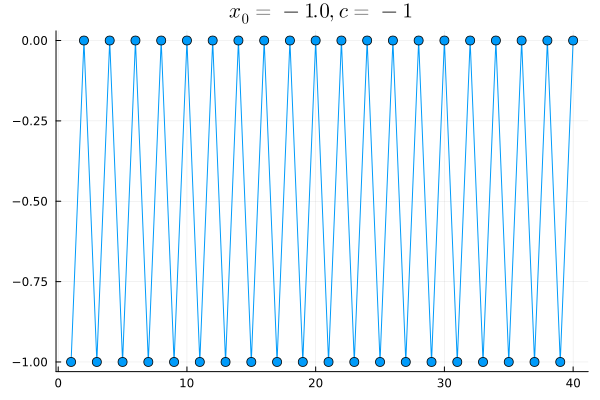
\includegraphics[width=\linewidth]{graphs/5.png}
		\end{subfigure}
		\begin{subfigure}[b]{\v\linewidth}
			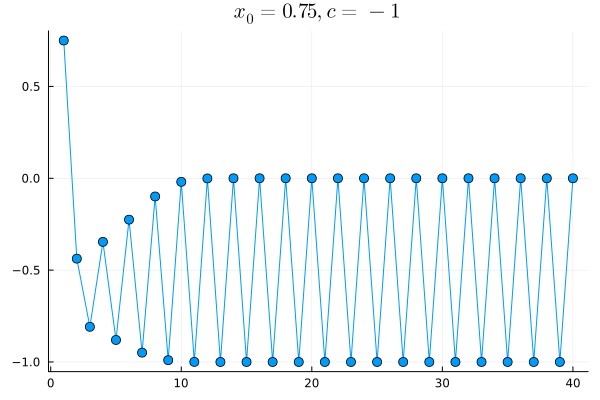
\includegraphics[width=\linewidth]{graphs/6.png}
		\end{subfigure}
		\begin{subfigure}[b]{\v\linewidth}
			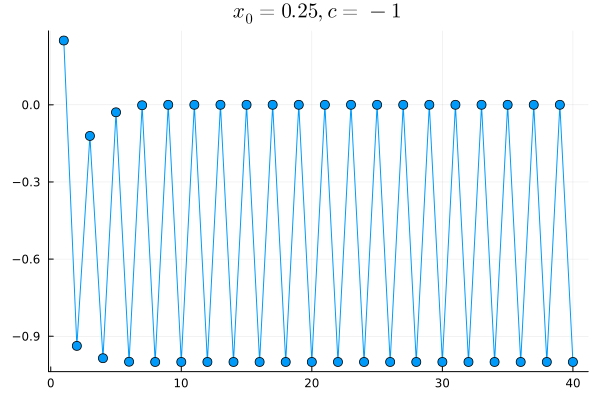
\includegraphics[width=\linewidth]{graphs/7.png}
		\end{subfigure}
	\end{figure}
\subsection*{Wnioski}

\end{document}